
%%%%%%%%%%%%%%%%%%%%%%%%%%%%%%%%%%%%%%%%%%%%%%%%%%%%%%%%%%%%
%%  This Beamer template was created by Cameron Bracken.
%%  Anyone can freely use or modify it for any purpose
%%  without attribution.
%%
%%  Last Modified: January 9, 2009
%%

\documentclass[xcolor={x11names,table},compress,svgnames,mathserif]{beamer}

%% General document %%%%%%%%%%%%%%%%%%%%%%%%%%%%%%%%%%
\usepackage{graphicx}
\usepackage{tikz}
\usetikzlibrary{decorations.fractals}
%\usepackage{lmodern}
\usepackage{animate}
\usepackage{movie15}
\usepackage{bm}
\usepackage{pifont}
\usepackage{empheq}
\usepackage[many]{tcolorbox}
\usepackage{smartdiagram}
\usepackage[customcolors]{hf-tikz}
\usepackage{dashrule} % for dotted vertical line
%\usepackage{flexisym}

\usepackage[absolute,overlay]{textpos}

\pgfdeclarehorizontalshading{section shading}{2cm}{
color(0cm)=(LightSlateGrey);
color(2cm)=(gray!7);
color(3cm)=(LightSlateGrey!15)
}

% Custom block environment
% Custom block environment
\newenvironment<>{varblock}[2][.9\textwidth]{%
  \setlength{\textwidth}{#1}
  \begin{actionenv}#3%
    \def\insertblocktitle{#2}%
    \par%
    \usebeamertemplate{block begin}}
  {\par%
    \usebeamertemplate{block end}%
  \end{actionenv}}

% boxed equaton
\usepackage[many]{tcolorbox}
%\tcbuselibrary{skins}

\tcbset{highlight math style={enhanced,
  colframe=red!60!black,colback=yellow!50!white,arc=4pt,boxrule=1pt,
  }}

\newtcbox{\mybox}[1][]{nobeforeafter,math upper,tcbox raise base,
  enhanced,frame hidden,boxrule=0pt,interior style={top color=green!10!white,
  bottom color=green!10!white,middle color=green!50!yellow},
  fuzzy halo=1pt with green,drop large lifted shadow,#1}

%%%%%%%%%%%%%%%%%%%%%%%%%%%%%%%%%%%%%%%%%%%%%%%%%%%%%%

\usetikzlibrary{shapes,arrows}
\usetikzlibrary{positioning,decorations.pathreplacing}
% Define block styles
\tikzstyle{decision} = [diamond, draw, fill=purple!20, 
    text width=5.0em, text badly centered, node distance=3cm, inner sep=0pt]
\tikzstyle{block} = [rectangle, draw=none, fill=blue!20, anchor=north, 
    text width=9.0em, text centered]
    \tikzstyle{blockr} = [rectangle, draw, fill=blue!20, 
    text width=9.0em, text centered, rounded corners]
\tikzstyle{line} = [draw, -latex']
\tikzstyle{cloud} = [draw=none, ellipse,fill=purple!20, node distance=3cm,
    minimum height=2em]
    

%% Beamer Layout %%%%%%%%%%%%%%%%%%%%%%%%%%%%%%%%%%
\useoutertheme[subsection=false,shadow]{miniframes}
\useinnertheme{default}
%\usefonttheme{serif}
\usepackage{palatino}
\usepackage{xcolor}
\usepackage{amsmath}
\newcommand{\angstrom}{\textup{\AA}}

\setbeamerfont{title like}{shape=\scshape}
\setbeamerfont{frametitle}{shape=\scshape}
\setbeamertemplate{itemize items}[triangle] % if you wnat a circle
\setbeamertemplate{itemize subitem}[triangle]
\setbeamertemplate{navigation symbols}{}
%\setbeamertemplate{footline}[frame number]

\setbeamercolor{footlinecolor}{fg=white,bg=DeepSkyBlue4}
\defbeamertemplate*{footline}{infolines theme}
{
  \leavevmode%
  \hbox{%
  \begin{beamercolorbox}[wd=.333333\paperwidth,ht=2.25ex,dp=1ex,center]{footlinecolor}
 % {author in head/foot}%
    \usebeamerfont{author in head/foot}\insertshortauthor
   % \usebeamerfont{author in head/foot}\insertshortauthor~~(\insertshortinstitute)
  \end{beamercolorbox}%
  \begin{beamercolorbox}[wd=.333333\paperwidth,ht=2.25ex,dp=1ex,center]{title in head/foot}%
    \usebeamerfont{title in head/foot}\insertshorttitle
  \end{beamercolorbox}%
  \begin{beamercolorbox}[wd=.333333\paperwidth,ht=2.25ex,dp=1ex,right]{footlinecolor}
  %{date in head/foot}%
   % \usebeamerfont{date in head/foot}\insertshortdate{}\hspace*{2em}
    \usebeamerfont{date in head/foot}{manav.vohra@vanderbilt.edu}\hspace*{2em}
    \insertframenumber{} / \inserttotalframenumber\hspace*{2ex} 
  \end{beamercolorbox}}%
  \vskip0pt%
}
%\setbeamercolor{section in head/foot}{fg=white, bg=DeepSkyBlue4}

\setbeamercolor*{lower separation line head}{bg=DeepSkyBlue4} 
\setbeamercolor*{normal text}{fg=black,bg=white} 
\setbeamercolor*{alerted text}{fg=red} 
\setbeamercolor*{example text}{fg=black} 
\setbeamercolor*{structure}{fg=black} 
 
\setbeamercolor*{palette tertiary}{fg=black,bg=black!10} 
\setbeamercolor*{palette quaternary}{fg=black,bg=black!10} 

\renewcommand{\(}{\begin{columns}}
\renewcommand*\footnoterule{}
\renewcommand{\)}{\end{columns}}
\newcommand{\<}[1]{\begin{column}{#1}}
\renewcommand{\>}{\end{column}}

\newcommand*\subitem{%
  \item[\color{DeepSkyBlue4}\scalebox{0.6}{\ding{228}}]}
  
  \newcommand*\subitemtwo{%
  \item[\color{LightSlateGrey!15}\scalebox{0.6}{\ding{228}}]}

\newcommand*\myitem{%
  \item[\color{DeepSkyBlue4}\scalebox{0.6}{\ding{110}}]}
 
  \newcommand*\myitemtwo{%
  \item[\color{LightSlateGrey!15}\scalebox{0.6}{\ding{110}}]}
  
\newcommand*\Myitem{%
  \item[\color{DeepSkyBlue4}\scalebox{0.9}{\ding{42}}]}
  
\newcommand{\be}{\begin{equation}}
\newcommand{\ee}{\end{equation}}
\newcommand{\bea}{\begin{eqnarray}}
\newcommand{\eea}{\end{eqnarray}}
\newcommand{\p}{\partial}
\def\ol{\overline}
\def\no{\noindent}
\def\Vb{{\cal V}}
\def\Qd{\dot{Q}}
%\DeclareMathSymbol{\ast}{\mathbin}{symbols}{"03}
 \newcommand{\argmax}{\operatornamewithlimits{arg\,max}}
 

%---------------------QUOTATION--------------------------
\usepackage{etoolbox}
%\usepackage[svgnames]{xcolor}
\usepackage{framed}

% conditional for xetex or luatex
\newif\ifxetexorluatex
\ifxetex
  \xetexorluatextrue
\else
  \ifluatex
    \xetexorluatextrue
  \else
    \xetexorluatexfalse
  \fi
\fi
%
\ifxetexorluatex%
  \usepackage{fontspec}
  \usepackage{libertine} % or use \setmainfont to choose any font on your system
  \newfontfamily\quotefont[Ligatures=TeX]{Linux Libertine O} % selects Libertine as the quote font
\else
  \usepackage[utf8]{inputenc}
  \usepackage[T1]{fontenc}
  %\usepackage{libertine} % or any other font package
  \newcommand*\quotefont{\fontfamily{LinuxLibertineT-LF}} % selects Libertine as the quote font
\fi

\newcommand*\quotesize{30} % if quote size changes, need a way to make shifts relative
% Make commands for the quotes
\newcommand*{\openquote}
   {\tikz[remember picture,overlay,xshift=-3ex,yshift=-0.5ex]
   \node (OQ) {\quotefont\fontsize{\quotesize}{\quotesize}\selectfont``};\kern0pt}

\newcommand*{\closequote}[1]
  {\tikz[remember picture,overlay,xshift=-15ex,yshift={#1}]
   \node (CQ) {\quotefont\fontsize{\quotesize}{\quotesize}\selectfont''};}

% select a colour for the shading
\colorlet{shadecolor}{Azure}

\newcommand*\shadedauthorformat{\emph} % define format for the author argument

% Now a command to allow left, right and centre alignment of the author
\newcommand*\authoralign[1]{%
  \if#1l
    \def\authorfill{}\def\quotefill{\hfill}
  \else
    \if#1r
      \def\authorfill{\hfill}\def\quotefill{}
    \else
      \if#1c
        \gdef\authorfill{\hfill}\def\quotefill{\hfill}
      \else\typeout{Invalid option}
      \fi
    \fi
  \fi}
% wrap everything in its own environment which takes one argument (author) and one optional argument
% specifying the alignment [l, r or c]
%
\newenvironment{shadequote}[2][l]%
{\authoralign{#1}
\ifblank{#2}
   {\def\shadequoteauthor{}\def\yshift{-2ex}\def\quotefill{\hfill}}
   {\def\shadequoteauthor{\par\authorfill\shadedauthorformat{#2}}\def\yshift{2ex}}
\begin{snugshade}\begin{quote}\openquote}
{\shadequoteauthor\quotefill\closequote{\yshift}\end{quote}\end{snugshade}}


%%%%%%%%%%%%%%%%%%%%%%%%%%%%%%%%%%%%%%%%%%%%%%%%%%

\title[UQ: Nano-scale Phonon Heat Transfer]{\textbf{Characterizing the Uncertainties in Non-Equilibrium MD for Thermal Transport}}
\thispagestyle{empty}
\pgfsetfillopacity{0.9}
\setbeamercolor{title}{bg=DeepSkyBlue4,fg=white}


%\subtitle{SUBTITLE}
\author[M. Vohra and S. Mahadevan]{Manav Vohra$^{\dag}$, Sankaran Mahadevan$^{\dag}$ \\ \vspace{1mm}
Collaborators: Seungha Shin$^{\S}$, Ali Yousefzadi Nobakht$^{\S}$}
\vspace{-1mm}
\institute{$^{\dag}$Vanderbilt University\\ \vspace{1mm}
$^{\S}$University of Tennessee, Knoxville}

\date{\today}


\begin{document}


%___________________________NEW SLIDE______________________________________
{
\setbeamertemplate{headline}{}

\begin{frame}[noframenumbering]

\titlepage
\vspace{-21mm}
\centering
%\scriptsize Institute for Computational Engineering and Sciences\\ \vspace{1mm}
%The University of Texas at Austin \\ \vspace{6mm}

%\footnotesize Seminar at SCI, University of Utah \\ \vspace{2mm}


\end{frame}
}

%___________________________NEW SLIDE______________________________________

\section{\scshape Background}
\subsection{md}
\begin{frame}{Background}

\begin{itemize}

\myitem Classical MD is used to investigate heat transfer dominated by phonon-phonon interactions
in material systems.  
\begin{itemize}
	\item Commonly applied to study non-metallic systems like C, Si, and Ge. 
\end{itemize}
		\vspace{1mm}
\myitem Typically conducted under equilibrium conditions characterized by thermodynamic ensembles like 
	NVT, NVE, NPT, and $\mu$VT.
		\vspace{1mm}

\myitem Non-Equilibrium MD involves setting up thermostats in different regions to establish temperature
gradients.
		\begin{itemize} 
			\item Thermostatting introduces errors. 
		\end{itemize}
		\vspace{1mm}
\end{itemize}

	{\scshape Why MD$?$} 
	\begin{itemize}
			\Myitem Enables simulation of much larger systems compared to DFT 
			in a reasonable amount of time. \vspace{1mm}
			\Myitem Trends from MD are useful despite possible errors in estimates.  
	\end{itemize}


\end{frame}

%___________________________NEW SLIDE______________________________________

\section{\scshape Plan}
\subsection{plan}
\begin{frame}{Plan}


Part I: \textsc{Forward Problem}:

\begin{itemize}

\myitem Investigate error in predictions due to {\color{blue}size} of the material system and
{\color{blue}fluctuations} in thermal gradient.

\begin{itemize} 
\item Construct a {\color{blue}response surface} for the error. 
\end{itemize}

%\vspace{2mm}

\myitem Characterize the impact of uncertainty in inter-atomic potential on predictions. 

\begin{itemize}
\item Efficient construction of surrogates using NISP: aPSP, Sparse Basis, Active Subspaces
\item Examine sensitivity of estimates on parameters.
\end{itemize}

\end{itemize}

Part II: \textsc{Inverse Problem}:

\begin{itemize}

\myitem Calibrate critical parameters associated with the potential function in
a Bayesian setting.

\begin{itemize} 
\item Exploit the error response surface from Part I.  
\end{itemize}

\end{itemize}

\end{frame}

%___________________________NEW SLIDE______________________________________

\section{\scshape Problem Set-up}
\subsection{setup}
\begin{frame}{NEMD on a Silicon Bar}

\begin{columns}
	\begin{column}{0.5\textwidth}

\begin{center}
\begin{tikzpicture}
\node[fill=white,inner sep=0pt] 
{\rowcolors{1}{DeepSkyBlue!20}{DeepSkyBlue!5}
	\resizebox{\columnwidth}{!}{
  \begin{tabular}{|l|c|}\hline
	  Lattice Constant ($\angstrom$) & 5.43 \\
	  $W$, $H$ ($\angstrom$) & 117.94, 117.94 \\
	  Temperature (K) & 300 \\
	  $\Delta t$ (ps) & 0.0005 \\
	  BC & Periodic \\
	  Structure & Diamond \\
	  Potential & Stillinger-Weber \\
  \hline
  \end{tabular}%
	}
};
\end{tikzpicture}
\end{center}

\end{column}

\begin{column}{0.5\textwidth}

%\begin{center}
%        \animategraphics[autopause,poster=first,loop,height=0.60\textwidth]{5}
%        {./animation/snap}{0}{64}
%\end{center}

\vspace{-5mm}


\begin{figure}[htbp]
	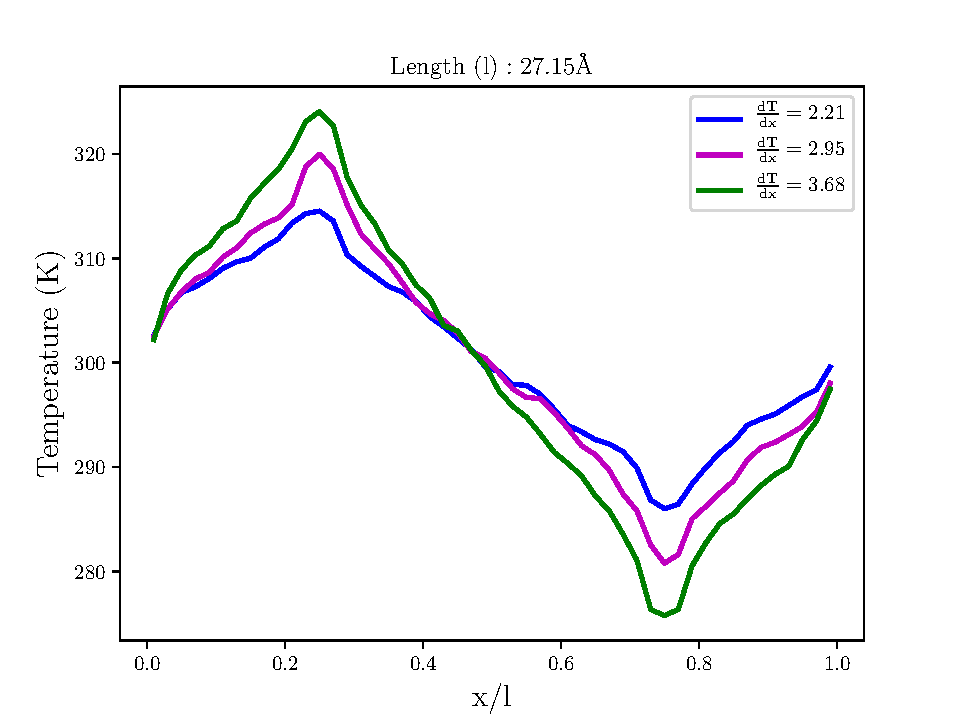
\includegraphics[width=0.9\textwidth]{./Figures/temp_plot}
\end{figure}

\end{column}
\end{columns}

\end{frame}

%___________________________NEW SLIDE______________________________________

\subsection{setup}
\begin{frame}{Optimize for Equilibration}

\vspace{-4mm}
\begin{center}

{\color{green}NVT} \hspace{5mm} $\rightarrow$ \hspace{5mm} {\color{cyan}NVE} \hspace{5mm}
$\rightarrow$ \hspace{5mm} {\color{magenta}NVE}
\\ \vspace{1mm}
\tiny \hspace{-5mm}[Eqilibrate system to 300 K] \hspace{1mm} [Equilibrate thermostats] \hspace{4mm}
 [Generate Data]

\end{center}

\vspace{3mm}
\textsc{Initial Runs}:

\begin{itemize}
\myitem Determine the time steps needed for equilibration at all stages. 
\vspace{2mm}

\myitem Select a {\color{blue}reasonable} width and height for the Si bar.
\begin{itemize}
\item Need to be in a regime where changes in width and height do not impact estimates significantly.   
\end{itemize}

\end{itemize}

\end{frame}


%___________________________NEW SLIDE______________________________________

\subsection{setup}
\begin{frame}{Selection of Width}

	\begin{columns}
	\begin{column}{0.5\textwidth}
		\begin{figure}[htbp]
			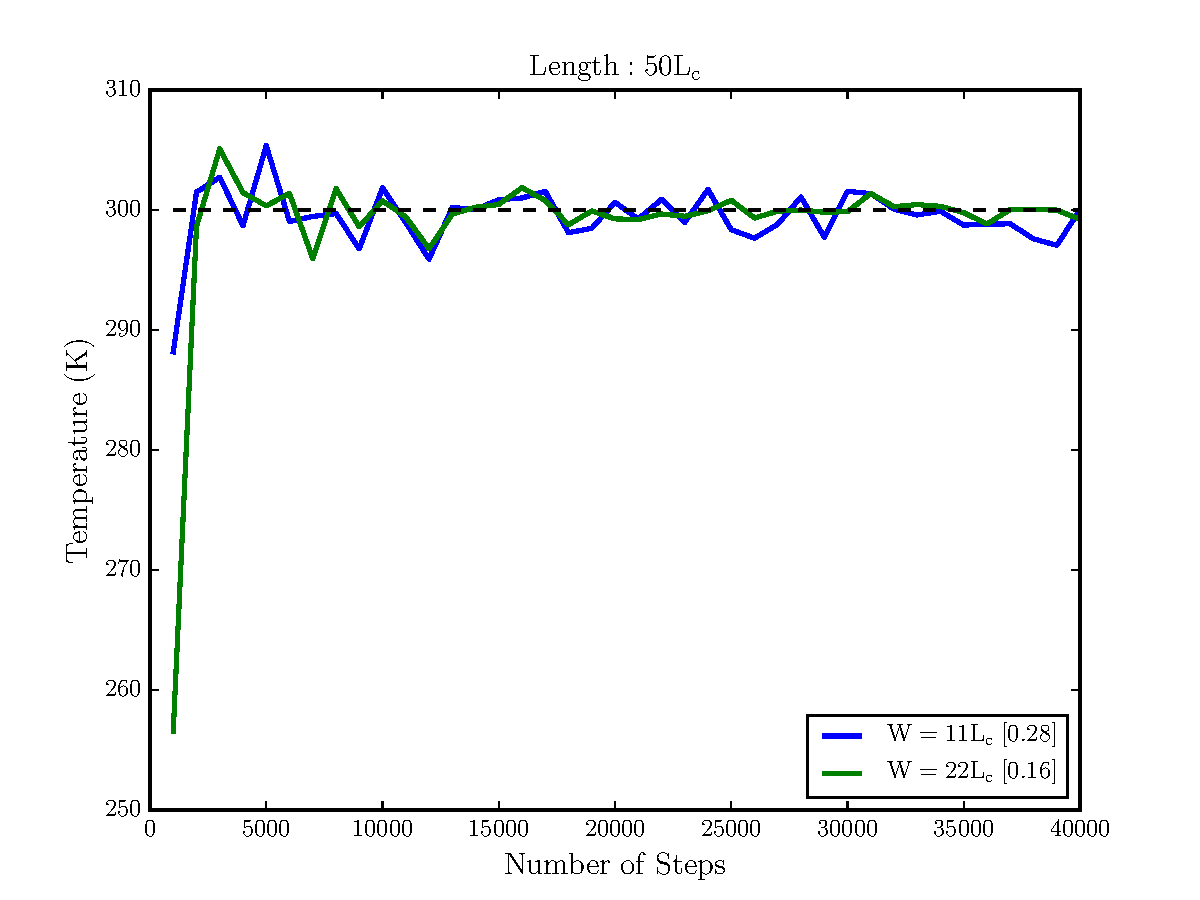
\includegraphics[width=0.85\textwidth]{./Figures/nvt_L50_wh_effect}
			\\
			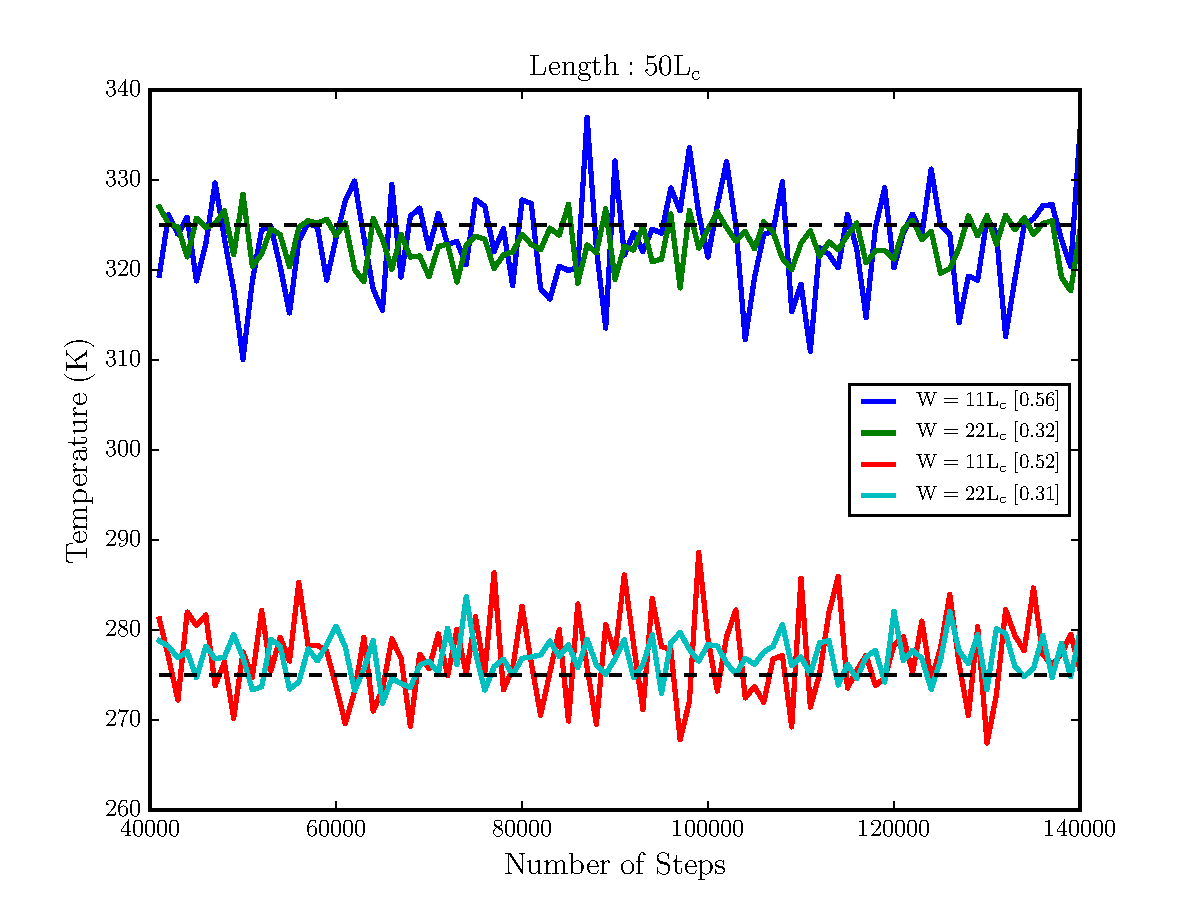
\includegraphics[width=0.85\textwidth]{./Figures/nve_L50_wh_effect}
			
		\end{figure}

	\end{column}
	\begin{column}{0.5\textwidth}
		\begin{figure}[htbp]
			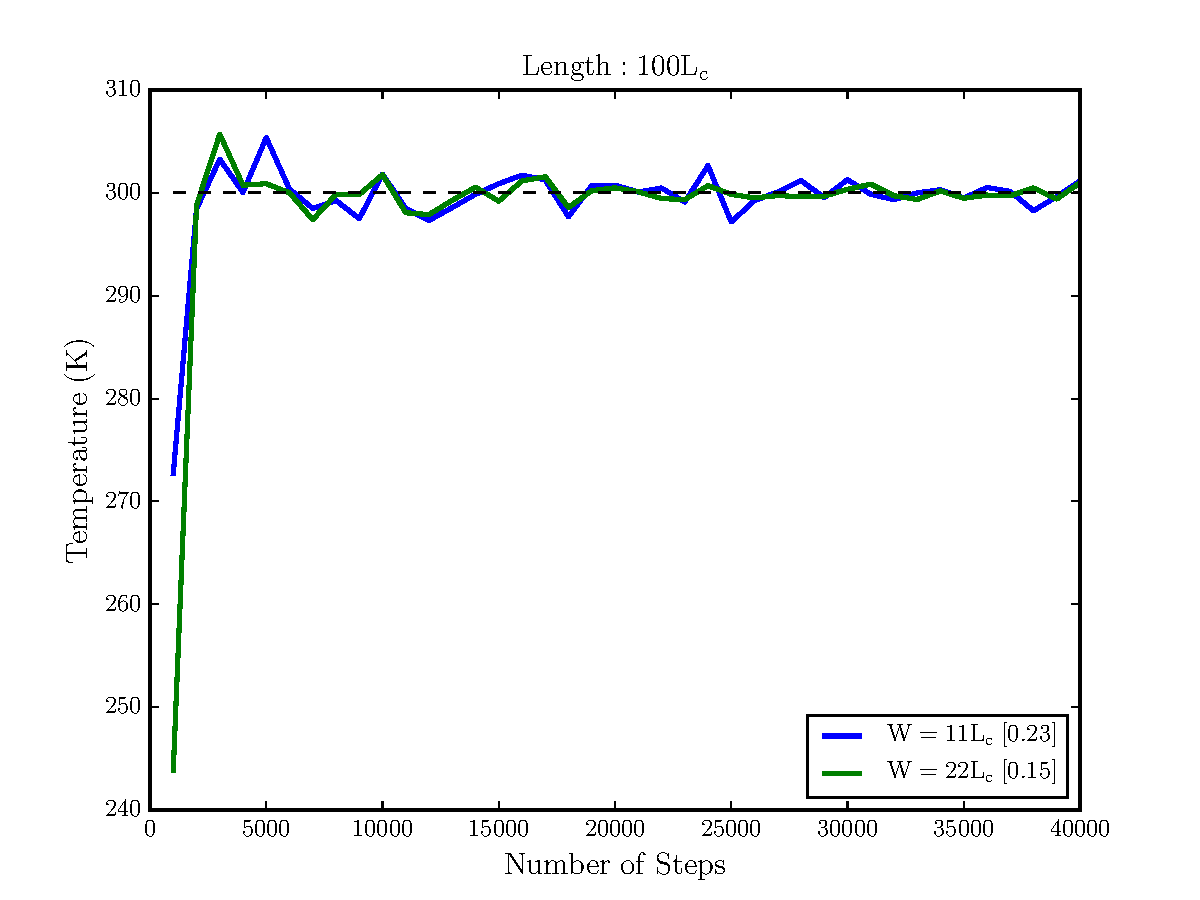
\includegraphics[width=0.85\textwidth]{./Figures/nvt_L100_wh_effect}
			\\
			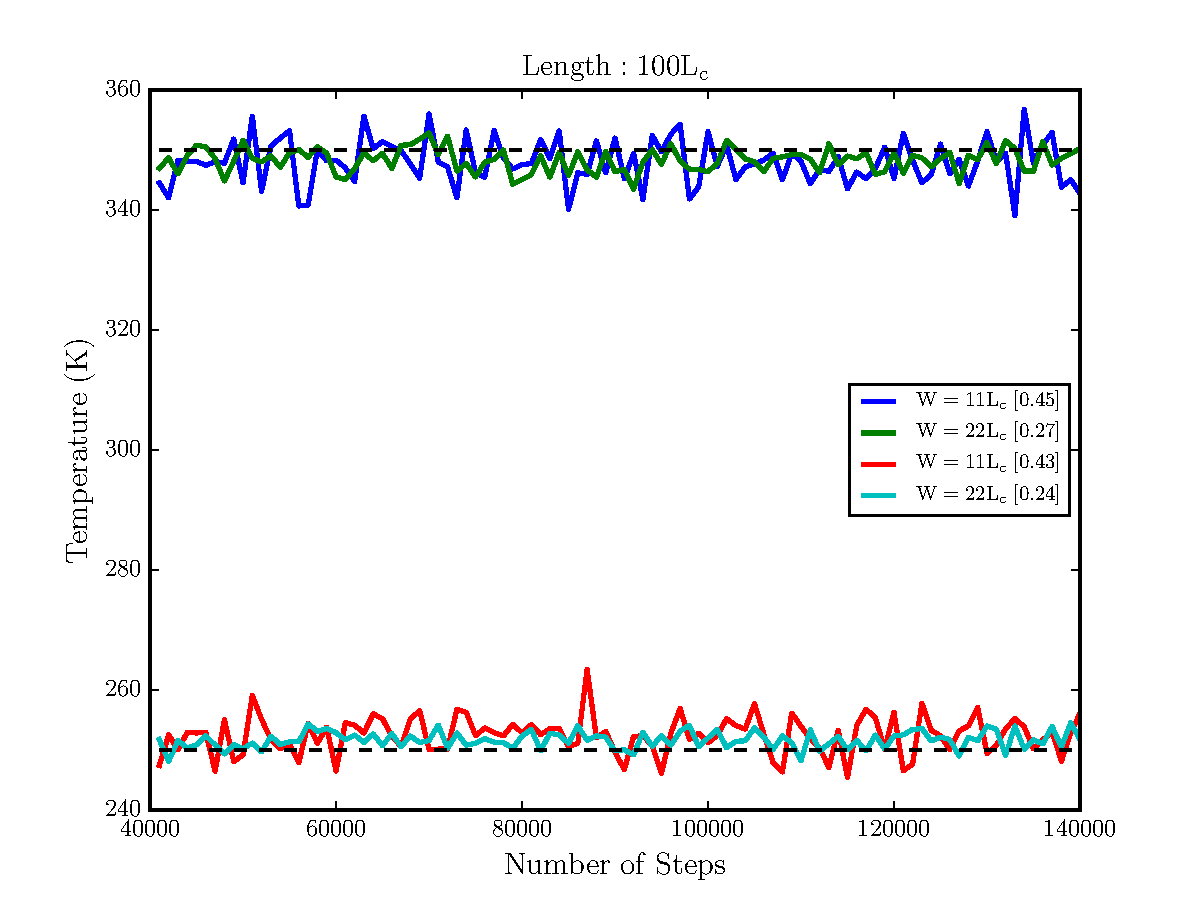
\includegraphics[width=0.85\textwidth]{./Figures/nve_L100_wh_effect}

		\end{figure}

	\end{column}
	
	\end{columns}

\end{frame}

%___________________________NEW SLIDE______________________________________

\subsection{setup}
\begin{frame}{Selection of Width}

	\begin{columns}
	\begin{column}{0.5\textwidth}
		\begin{figure}[htbp]
			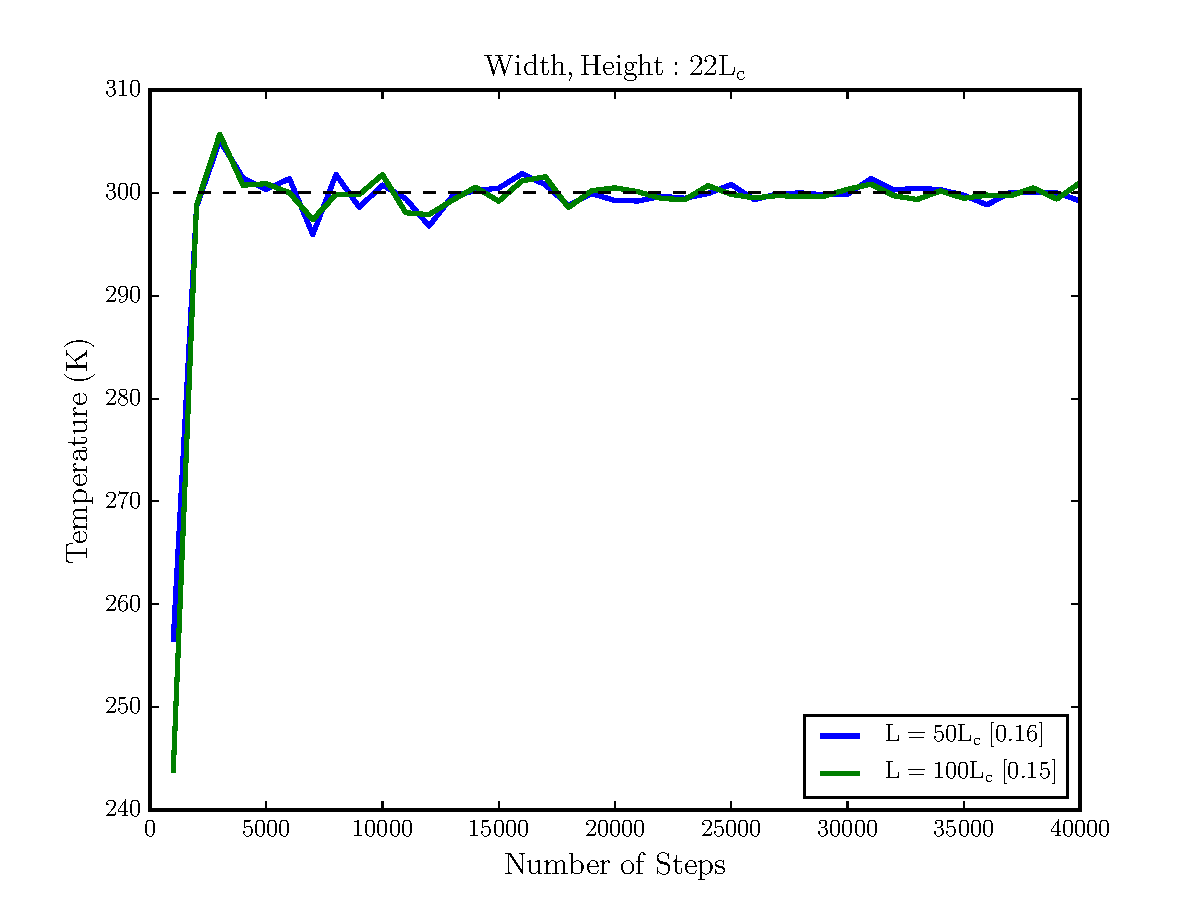
\includegraphics[width=1.0\textwidth]{./Figures/nvt_l_effect}
		\end{figure}

	\end{column}
	\begin{column}{0.5\textwidth}
		\begin{figure}[htbp]
			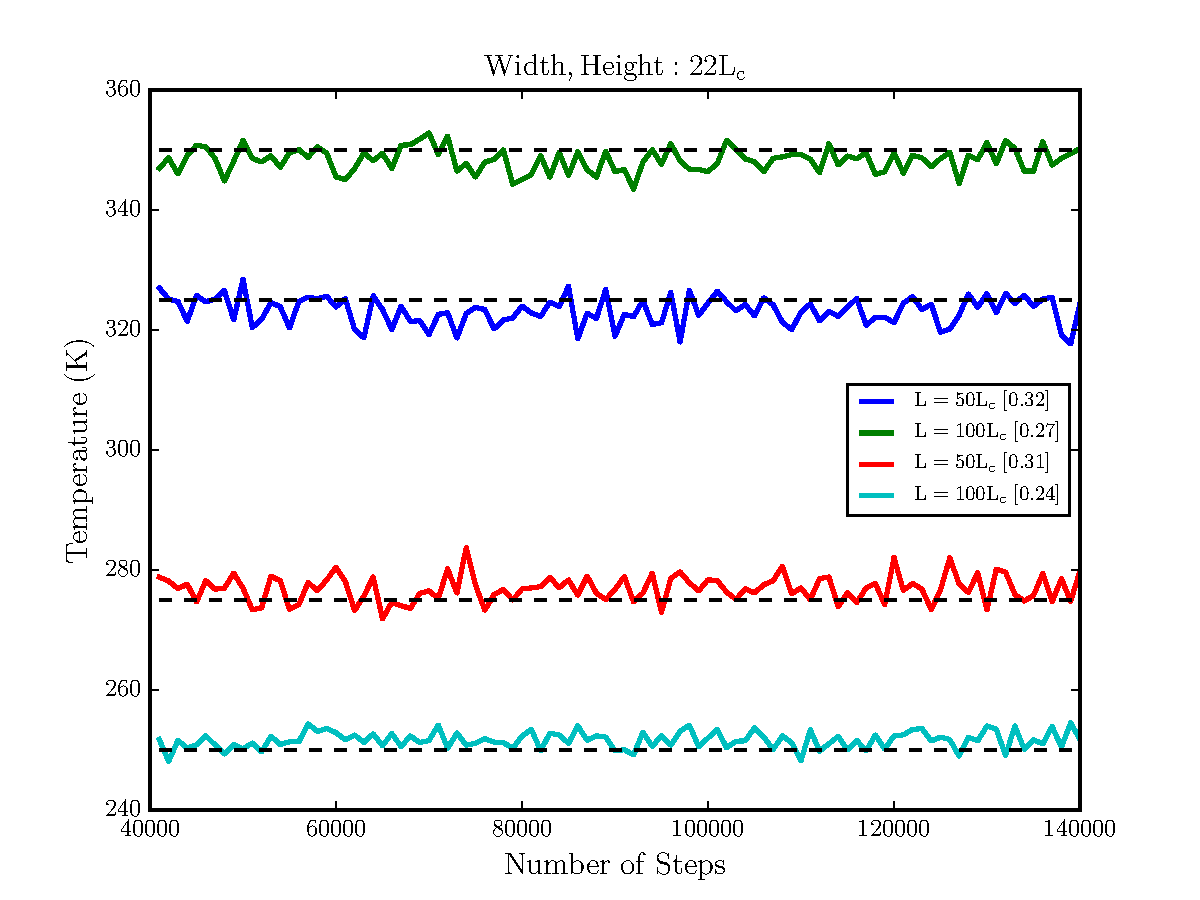
\includegraphics[width=1.0\textwidth]{./Figures/nve_l_effect}
		\end{figure}

	\end{column}
	
	\end{columns}

%\vspace{2mm}
\begin{itemize}

\myitem Norm of the fluctuations ($NF$) is computed using:

\begin{center}
\vspace{-5mm}

	\be 
            NF = \frac{1}{N}\left[\sum_k \left(T_k - T_{\{nvt,nve\}}\right)^{2}\right]^{\frac{1}{2}} \nonumber
        \ee

\end{center}

\myitem At $W$ = 21.72$L_c$, the effect of length on fluctuations seems to be minuscule. 
\end{itemize}

\end{frame}

%___________________________NEW SLIDE______________________________________

\section{\scshape Response Surface}
\subsection{err}
\begin{frame}{Need a Surrogate$?$}

\begin{columns}
\begin{column}{0.5\textwidth}

\begin{itemize}
\myitem \textsc{Objective}: Forward UQ, Sensitivity Analysis, calibration, Design
\vspace{2mm}
\myitem \textsc{Computational Effort}: Simulations are computationally intensive.
\vspace{2mm}
\myitem \textsc{Accuracy}: Can a surrogate represent the observable
with reasonable accuracy in the domain of interest$?$ 
\end{itemize}

\end{column}

\begin{column}{0.5\textwidth}

\begin{figure}[htbp]
	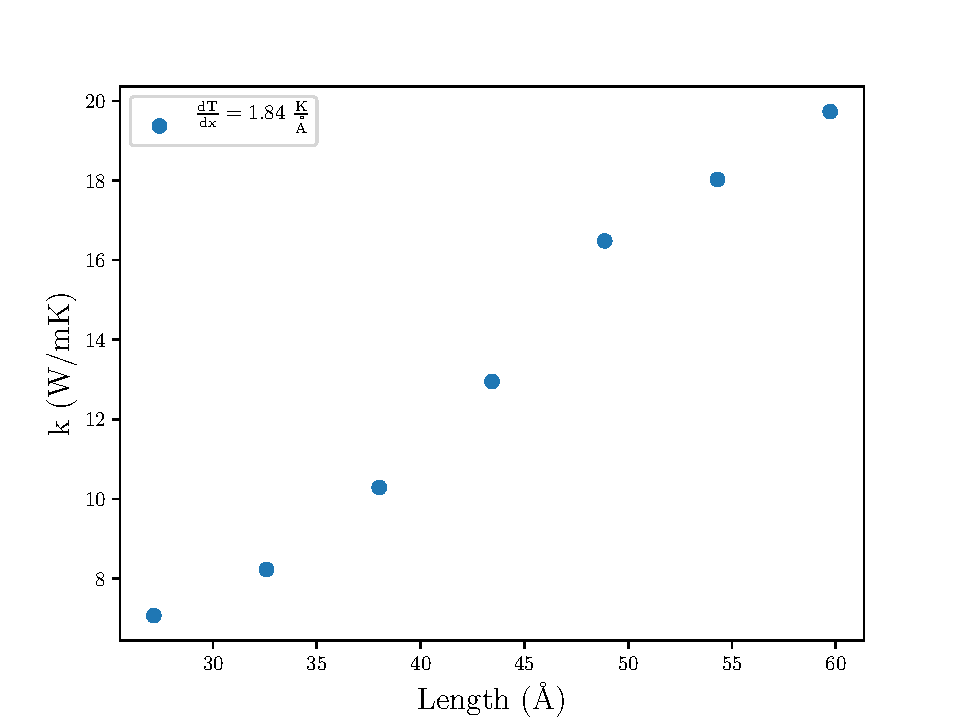
\includegraphics[width=1.0\textwidth]{./Figures/cond_size}
\end{figure}


\end{column}
\end{columns}

\end{frame}


%___________________________NEW SLIDE______________________________________

\subsection{err}
\begin{frame}{Model Realizations}

\begin{columns}

\begin{column}{0.5\textwidth}
\begin{center}
\begin{figure}[htbp]
  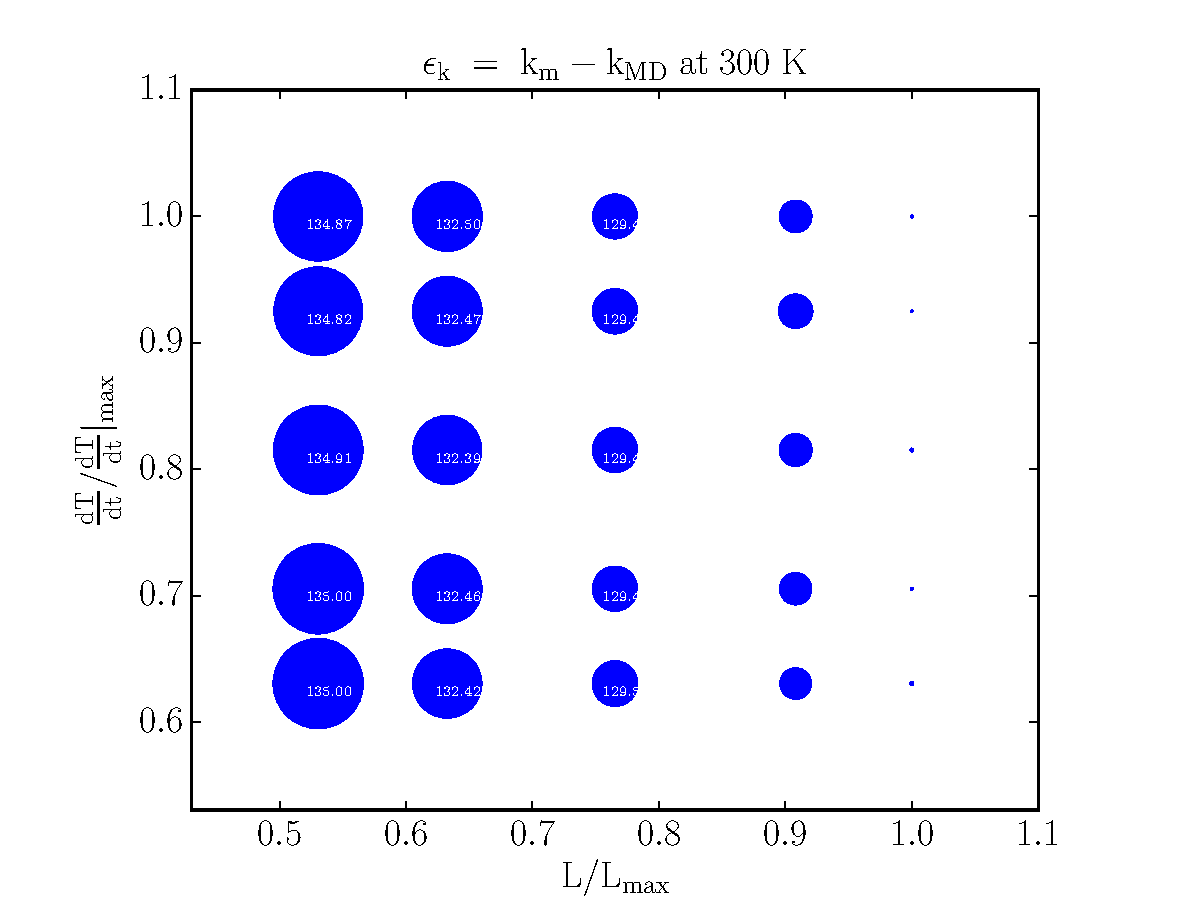
\includegraphics[width=1.2\textwidth]{./Figures/realz_quad300K}
\end{figure}
\end{center}
\end{column}
\hspace{-6mm}
\begin{column}{0.5\textwidth}
\begin{center}
\begin{figure}[htbp]
  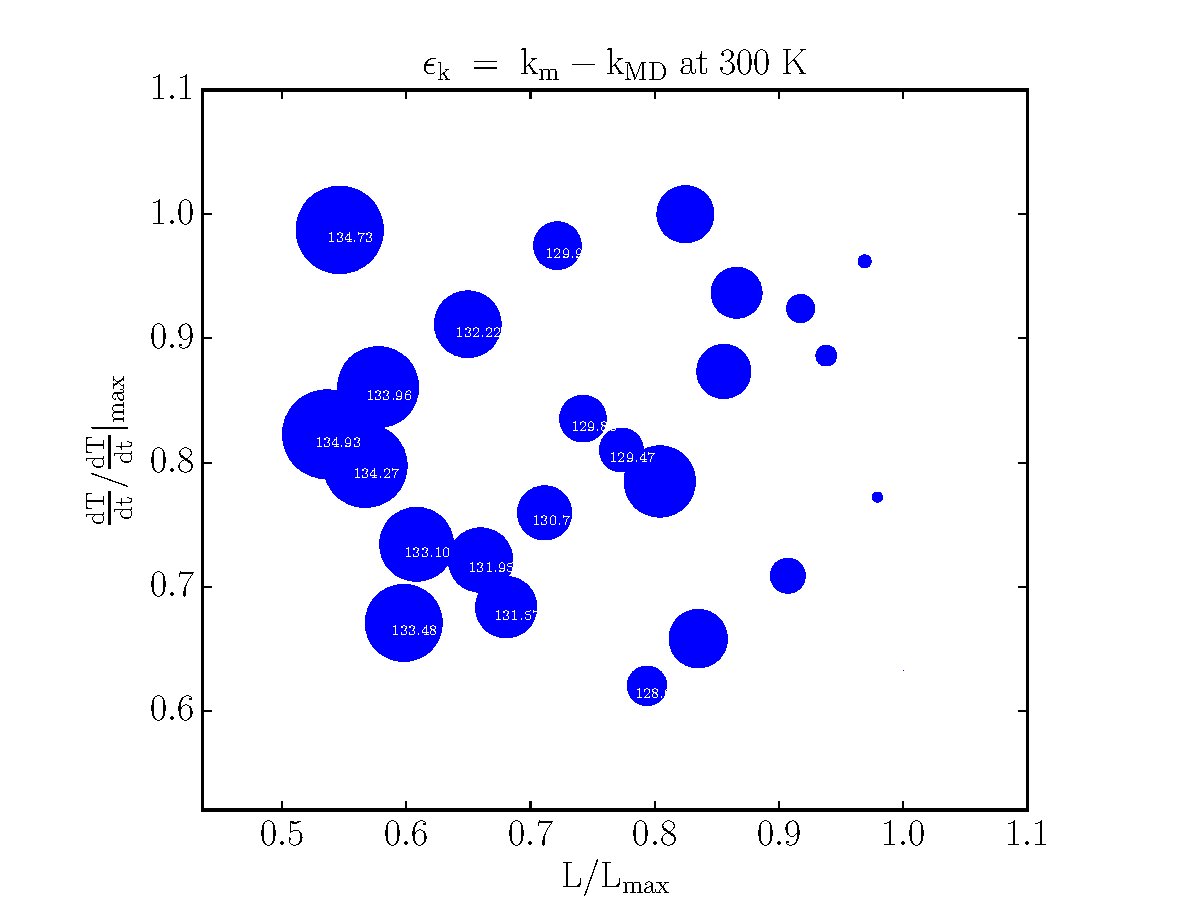
\includegraphics[width=1.2\textwidth]{./Figures/realz_sobol}
\end{figure}
\end{center}
\end{column}
\end{columns}

%\vspace{1mm}
\begin{itemize}
\myitem Model realizations at Gauss-Legendre quadrature nodes are used to
construct the PC surrogate.
\end{itemize}

\end{frame}


%___________________________NEW SLIDE______________________________________

\subsection{err}
%
\begin{frame}{PC Expansion}
%
\begin{columns}
\begin{column}{0.5\textwidth}

\begin{center}
\begin{empheq}[box=\tcbhighmath]{align}
  \kappa = \sum_j c_j\Psi_j(\xi_1,\xi_2) \nonumber
\end{empheq}

\tiny {$\kappa$: Thermal Conductivity, $j$: Multi-index}
\end{center}

\end{column}

\hspace{-5mm}
\begin{column}{0.5\textwidth}

\begin{figure}[htbp]
	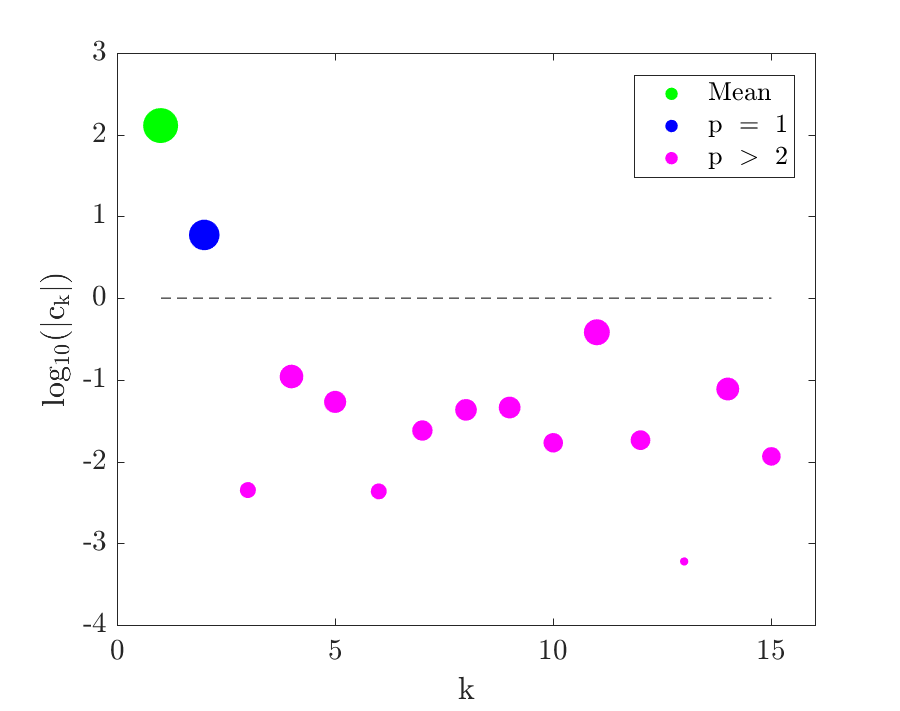
\includegraphics[width=1.2\textwidth]{./Figures/PCspectrum_300}
\end{figure}


\end{column}
\end{columns}

\vspace{1mm}
\begin{center}
\normalsize
$L$:~$\mathcal{U}[50L_c,100L_c]~(\angstrom)~~\rightarrow~~\xi_1: \mathcal{U}[-1,1]$ \\ \vspace{2mm}
$\frac{dT}{dx}$:~$\mathcal{U}[1.5/L_c,2.5/L_c]~(\frac{K}{\angstrom})~~\rightarrow~~\xi_2: \mathcal{U}[-1,1]$
\end{center}

\end{frame}


%___________________________NEW SLIDE______________________________________

\subsection{err}
%
\begin{frame}{Response Surface: $\epsilon(L,\frac{dT}{dx})$}
%
\begin{columns}
\begin{column}{0.5\textwidth}
\vspace{-8mm}
\begin{center}
\tiny{
\begin{empheq}[box=\tcbhighmath]{align}
  \epsilon = |\kappa_m - \kappa_{\tiny NEMD}| \nonumber
\end{empheq}
}
\tiny{$\kappa_m$: Measured Thermal Conductivity\\ $\kappa_{\tiny NEMD}$: MD Prediction}
\end{center}

\normalsize
\vspace{-2mm}
\textsc{Accuracy}:
\vspace{-2mm}

\begin{center}
\begin{figure}[htbp]
%\hspace{-5mm}
  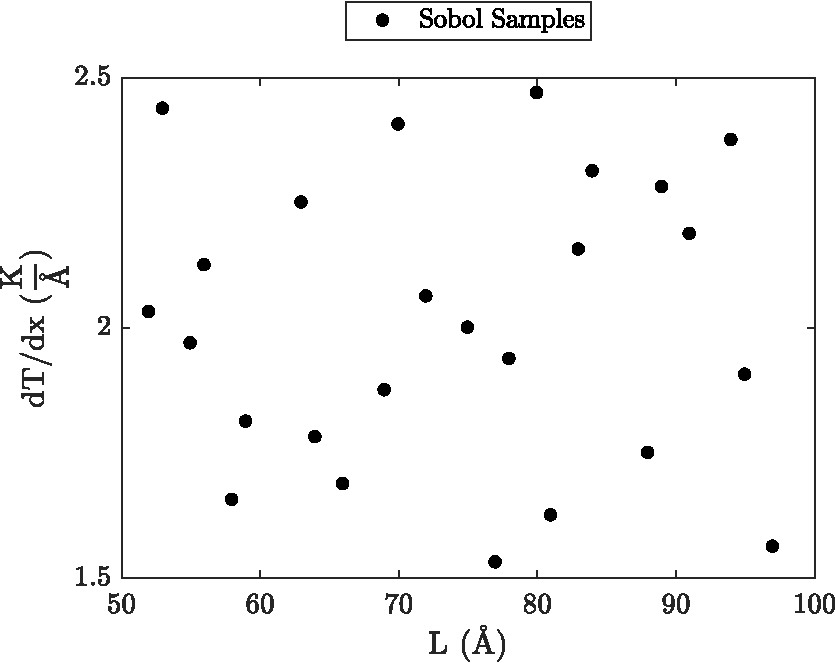
\includegraphics[width=0.65\textwidth]{./Figures/err2D_s}
\end{figure}

\vspace{-6mm}
%\tiny{
%\begin{empheq}[box=1.2\tcbhighmath]{align}
%  \alpha = \frac{\left[ \sum_j \left(\mathcal{G}\left(L(\xi_{1_j}),\frac{dT}{dx}(\xi_{2_j})\right) - \sum_k c_k\Psi_k(\xi_{1_j},\xi_{2_j})\right)^2\right]^{\frac{1}{2}}}{\left[\sum_j\left(\mathcal{G}\left(L(\xi_{1_j}),\frac{dT}{dx}(\xi_{2_j})\right)\right)^2\right]^{\frac{1}{2}}} \nonumber
%\end{empheq}
%}
\tiny{
\begin{empheq}[box=\tcbhighmath]{align}
  \epsilon = \frac{\left[ \sum_j \left(\mathcal{G}_M - \mathcal{G}_{PCE})\right)^2\right]^{\frac{1}{2}}}{\left[\left(\mathcal{G}_{M}\right)^2\right]^{\frac{1}{2}}} \approx 1.8\times10^{-3} \nonumber
\end{empheq}
}

\vspace{-3mm}
\tiny{
$\mathcal{G}_M$: Model Output\hspace{5mm}$\mathcal{G}_{PCE}$: PCE Estimate}
\end{center}

\end{column}

\begin{column}{0.5\textwidth}
\vspace{-10mm}
\begin{center}
\begin{figure}[htbp]

	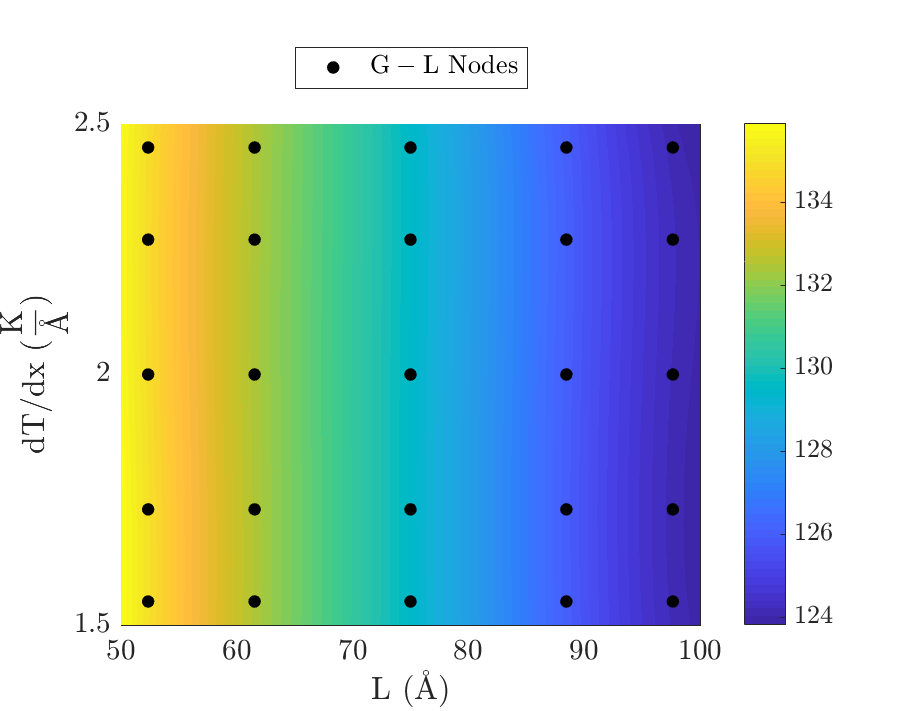
\includegraphics[width=0.8\textwidth]{./Figures/err2D_300}
	\\ \tiny (a) 300~K \\
	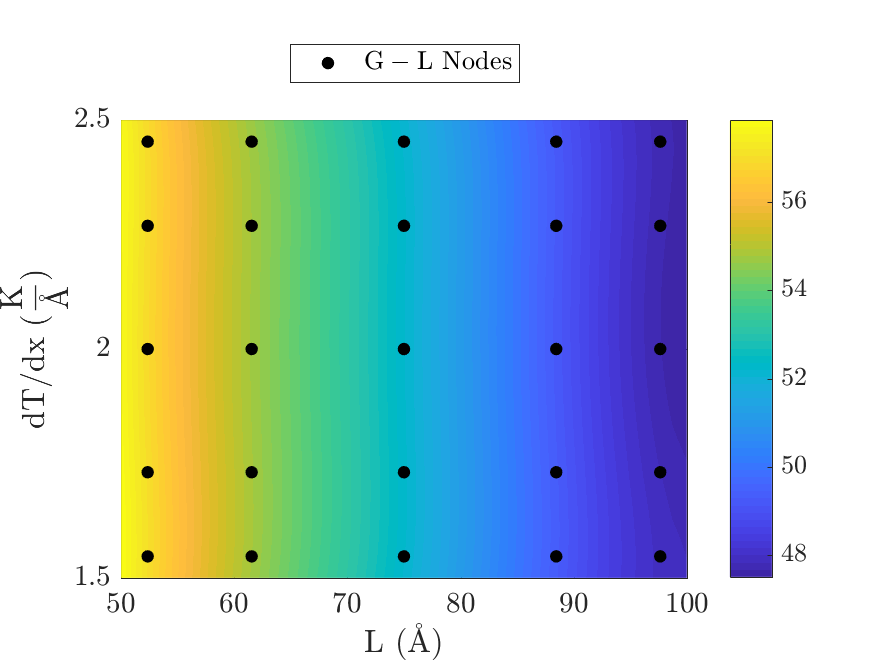
\includegraphics[width=0.8\textwidth]{./Figures/err2D_500}
	\\ \tiny (b) 500~K

\end{figure}
\end{center}


\end{column}
\end{columns}

\end{frame}

%___________________________NEW SLIDE______________________________________

\subsection{err}
%
\begin{frame}{Next Steps}

\begin{itemize}
\myitem Dimension reduction through Local Sensivity Analysis.
\vspace{2mm}
\myitem Estimate posterior distributions for significant potential function parameters.
\vspace{2mm}
\myitem Discover a potential active subspace.
\end{itemize}

\end{frame}














\end{document}
